\section{Demonstration and Test Case}

To demonstrate the functionality of the proposed system, a web-based application has been developed and deployed at:

\begin{center}
\url{https://mora-building.vercel.app/}
\end{center}

The application provides an interactive interface that allows users to configure scenarios, execute the optimization model, and visualize the resulting fire-response strategy in real time.

\subsection{Model Demonstration}

To illustrate the operation of the proposed optimization model, a simplified scenario representing a single floor of a small apartment building is used. The purpose of this demonstration is to validate that the outputs produced by the system comply with the model constraints and optimization objectives.

The floor is divided into a $3 \times 3$ grid of cells, where each cell represents a spatial zone within the building. This zone-based representation simplifies the modelling of fire spread, smoke propagation, and response team deployment.

The simulation is evaluated over four time periods ($t = 0, 1, 2, 3$). Each period represents a discrete operational time step (for example, 15 minutes or another appropriate emergency response interval). In this demonstration, the fire and smoke spread rates are assumed to be constant, meaning that they do not vary across time periods. As a result, the cell sizes remain unchanged and the following parameters remain fixed throughout the simulation:

\begin{itemize}
\item Fire arrival time for each cell
\item Smoke arrival time for each cell
\item Population density in each cell
\item Property value associated with each cell
\end{itemize}

Figure~\ref{fig:cell_parameters} illustrates the parameters used in the scenario.

\begin{figure}[h]
\centering
\includegraphics[width=\textwidth]figures/cell_parameters.png}
\caption{Cell parameters for the demonstration scenario. (a) Cell indexes, (b) Fire arrival time periods, (c) Smoke arrival time periods, (d) Population distribution, (e) Property value distribution}
\label{fig:cell_parameters}
\end{figure}

Based on the fire arrival time matrix, the fire initially starts in cell 5, which becomes the first high-risk fire zone. The smoke spreads faster than the fire; therefore, at the beginning cell 4 is also affected by the smoke from the fire in cell 5.

\subsubsection*{Response Resources}

Three different response team types are considered in the experiment:

\begin{itemize}
\item \textbf{Type A}: basic fire suppression unit (low cost, moderate suppression capability)
\item \textbf{Type B}: fire brigade unit capable of both suppression and rescue operations
\item \textbf{Type C}: specialized response unit with balanced suppression and rescue capabilities
\end{itemize}

In real-world situations, these resource types could represent, for example:

\begin{itemize}
\item \textbf{Type A}: hand crew firefighters
\item \textbf{Type B}: fire engines with rescue teams
\item \textbf{Type C}: aerial firefighting units or specialized rapid-response teams
\end{itemize}

Each resource type has a different suppression rate, rescue capability, and deployment cost, as summarized in Table~\ref{tab:resources}.

The minimum suppression rate required to contain the fire in each cell is illustrated in Figure~\ref{fig:suppression_requirement}, while the total available deployment budget is 30 units.

\begin{figure}[h]
\centering
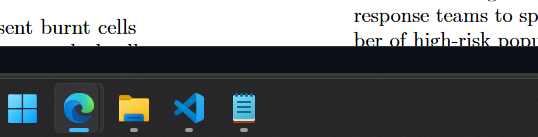
\includegraphics[width=0.6\textwidth]{figures/suppression_requirement.png}
\caption{Minimum suppression requirement for each cell}
\label{fig:suppression_requirement}
\end{figure}

\subsubsection*{Optimization Objective}

The optimization model determines how to allocate available response teams to different cells over time. The objective is to:

\begin{enumerate}
\item Minimize the total population exposed to fire and smoke risk
\item Minimize the total property value lost due to burnt cells
\item Minimize the total deployment cost of response resources
\end{enumerate}

In this formulation, property loss is directly associated with burnt cells, meaning that minimizing the number of burnt cells directly reduces the total value loss.

\subsubsection*{Simulation Results}

The optimal solution obtained from the model is illustrated in Figure~\ref{fig:simulation_results}.

In the visualization:

\begin{itemize}
\item Red dots represent fire high-risk cells
\item Orange dots represent smoke high-risk cells
\item Blue dots represent cells where fire has been successfully suppressed
\item Green dots represent cells where occupants have been rescued
\item Black dots represent burnt cells
\item Grey dots represent smoked cells
\end{itemize}

\subsubsection*{Time Step ($t = 0$)}

At the initial time step, cell 5 is both a fire and smoke high-risk cell. However, only one Type C unit is available at this time.

Because the suppression capability of a Type C unit (suppression rate = 2) is lower than the minimum suppression requirement of cell 5, the model determines that deploying this unit to cell 5 would not successfully contain the fire.

Instead, the model recommends allocating the Type C unit to cell 4, which is under smoke risk but still accessible for early intervention.

Since the remaining resources are unavailable at this time step, no suppression action is performed on cell 5. Consequently, by the next period the fire continues to spread.

\subsubsection*{Time Step ($t = 1$)}

By $t = 1$, cell 5 becomes fully burnt, and the fire spreads to neighboring cells 1, 2, 4, and 8.

At this stage, additional resources become available. The optimization model recommends:

\begin{itemize}
\item Deploying one Type A unit to cell 4
\item Deploying one Type A unit and one Type B unit to cell 2
\end{itemize}

This allocation enables:

\begin{itemize}
\item Successful fire suppression in cell 2
\item Rescue of the occupants located in that cell
\end{itemize}

However, cell 4 receives only a Type A unit, which has fire suppression capability but no rescue capability. Therefore, although the fire is partially controlled, the occupants in that cell cannot be rescued.

During this period, cells 1 and 8 become fully burnt and smoked due to the continued fire spread.

\subsubsection*{Time Step ($t = 2$)}

At the next time step, the fire spreads further to cells 0 and 3.

The model allocates resources as follows:

\begin{itemize}
\item One Type B unit is deployed to cell 0
\item One Type A unit and one Type C unit are deployed to cell 3
\end{itemize}

These deployments provide sufficient suppression capacity to contain the fire in these cells and prevent further spread.

\subsubsection*{Final State ($t = 3$)}

By the final time step, all active fire and smoke risks have been contained, and no further resource deployments are required.

The final outcome of the simulation shows:

\begin{itemize}
\item Several cells successfully suppressed
\item Some occupants rescued
\item A limited number of cells burnt due to early fire propagation before sufficient resources became available
\end{itemize}

In summary, this demonstration illustrates how the proposed optimization model dynamically allocates emergency response resources across space and time.

The model generates recommendations for deploying response teams to specific cells in order to reduce the number of high-risk population zones, minimize property value losses caused by fire spread, and utilize response resources efficiently under budget and availability constraints.

The interactive visualization shown in Figure~\ref{fig:simulation_results} highlights both the hazard propagation process (left grid) and the results of suppression and rescue actions (right grid), providing a clear understanding of how the optimization model supports decision-making during emergency response operations.